% =============================================================================
% CAPÍTULO 3 — volta 1 (AGENTS.md §6): a forma que o relógio desenha.
%
% O fracasso que o abre, com número na mão: levado à carga elétrica diária da Dinamarca no
% mesmo orçamento de um alarme por ano, o vigia do capítulo 2 dispara 4,2 vezes por ano e
% TODOS os alarmes caem em fim de semana — 8 sábados e 13 domingos, nenhum dia útil.
%
% O princípio: o calendário é uma partição dos dias em células, e o corte se ergue dentro da
% célula. O preço: a partição divide a memória por C, e o orçamento mais fino passa de
% 1/(n+1) para C/(n+C). O controle é o índice americano, onde não há calendário semanal.
%
% Medição: lab/experimentos/E04_calendario.ipynb. Figuras: figuras/E04_calendario_*.
% =============================================================================

\chapter{O dia da semana}
\label{cap:calendario}

\section{O domingo não é uma mudança}

O capítulo anterior deixou um vigia com orçamento declarado, e a conta dele se apoia numa
hipótese: os dias são trocáveis, qualquer ordem é igualmente provável. Numa série de retornos
de mercado essa hipótese é razoável durante meses seguidos. Existem séries em que ela é falsa
todo sábado, e não por acidente.

O consumo de energia elétrica de um país é uma delas. São \numCalendarioSerieDias{} dias da
Dinamarca, de \numCalendarioSerieInicio{} a \numCalendarioSerieFim, com o consumo medido a cada
dia. Aplicado a essa série no mesmo orçamento de um alarme por ano, o vigia do capítulo
anterior disparou \numCalendarioCruAlarmes{} vezes, ou \numCalendarioCruAlarmesAno{} por ano
--- quase o triplo do que havia declarado. E os alarmes têm todos a mesma cara:
\numCalendarioCruFimDeSemanaPct\% caem em fim de semana, \numCalendarioCruSabado{} sábados e
\numCalendarioCruDomingo{} domingos, com \numCalendarioCruSexta{} sextas e nenhum outro dia
útil.

Um alarme que só soa no fim de semana não está relatando o mundo. Está relatando o calendário,
e o calendário não muda.

\section{O tamanho do calendário}

O domingo consome \numCalendarioDomingoPct\% menos que o dia médio, e o padrão se repete em todas as semanas dos cinco anos. Vale medir o tamanho desse perfil
em cada série, porque é ele que decide se o calendário atrapalha o vigia. A medida é a
distância entre o dia mais cheio e o mais vazio da semana, contada em desvios-padrão do dia.

\begin{table}[htbp]
  \centering
  \begin{tabular}{lr}
    \hline
    série & amplitude do perfil semanal \\
     & (desvios-padrão do dia) \\
    \hline
    carga da Dinamarca & \numCalendarioAmplitudeCarga \\
    carga da França & \numCalendarioAmplitudeFr \\
    carga da Espanha & \numCalendarioAmplitudeEs \\
    carga da Polônia & \numCalendarioAmplitudePl \\
    carga da Áustria & \numCalendarioAmplitudeAt \\
    \hline
    índice S\&P 500 & \numCalendarioAmplitudeIndice \\ % numeros-ok: nome próprio, não medição
    \hline
  \end{tabular}
  \caption{O tamanho do calendário, medido. Nas cargas europeias a semana desenha mais de um
    desvio-padrão; no índice americano ela desenha quase nada.}
  \label{tab:perfil}
\end{table}

A carga dinamarquesa tem \numCalendarioAmplitudeCarga{} desvios-padrão entre o dia mais cheio e
o mais vazio, e as praças vizinhas vão de \numCalendarioAmplitudeFr{} a
\numCalendarioAmplitudePl. O índice acionário americano, medido do mesmo jeito, fica em
\numCalendarioAmplitudeIndice. É uma razão de dezenas, e ela separa dois casos que a mesma
regra de vigilância trata de formas opostas.

\section{Ler o dia no seu próprio dia}

O conserto é de uma linha: em vez de comparar hoje com os últimos \numCalendarioJanela{} dias,
compara-se hoje com os últimos \numCalendarioJanela{} dias \emph{do mesmo dia da semana}. O
calendário entra na conta como o que ele é, uma partição dos dias em células, e o corte passa a
ser erguido dentro da célula: o domingo mede o domingo, a terça mede a terça.

Vale dizer o que essa leitura tem de conservador. Com uma célula só --- todos os dias iguais
--- ela é exatamente o vigia do capítulo anterior, alarme por alarme, porque a célula única
recebe a janela inteira. A partição não inventa instrumento novo; ela declara em que célula
cada dia é julgado.

O que se ganha é imediato e o que se paga vem depois. Depois da partição, os alarmes deixam de
ser o fim de semana: caem em \numCalendarioSemanaFimDeSemanaPct\% em fim de semana, contra os
\numCalendarioCruFimDeSemanaPct\% da leitura crua, e espaçam-se pelos sete dias. O vigia
começou a falar de consumo em vez de falar de calendário.

\section{A partição divide a memória}

O preço aparece na conta do capítulo anterior, lida célula por célula. Repartida por $C$ células, a janela de \numCalendarioJanela{} dias deixa de ser memória inteira de cada decisão: cada célula recebe $n/C$ dias, e o alarme mais raro que uma célula
consegue declarar é $1/(n/C + 1)$. Somando as sete células da semana, o orçamento mais fino
que a leitura inteira consegue declarar é $C/(n+C)$ por dia --- e sete células tornam o alarme
quase sete vezes mais frequente do que a leitura crua.

Cada célula que se decide ler multiplica o orçamento, e a medição acompanha. Repartir a janela
entre sete dias da semana dá 
\numCalendarioSemanaDiasPorCelula{} dias a cada célula; entre vinte
e oito partes, dá nove; entre oitenta e quatro, dá três. A memória por decisão encolhe, e o
alarme mais raro que ela consegue declarar engorda junto.

\begin{table}[htbp]
  \centering
  \begin{tabular}{lr}
    \hline
    leitura & alarmes por ano \\
     & (o que a memória declara) \\
    \hline
    o dia sozinho & \numCalendarioCruAlarmesAno\ (\numCalendarioCruPisoAno) \\
    o dia da semana & \numCalendarioSemanaAlarmesAno\ (\numCalendarioSemanaPisoAno) \\
    o dia e a estação & \numCalendarioTrimestreAlarmesAno\ (\numCalendarioTrimestrePisoAno) \\
    o dia e o mês & \numCalendarioMesAlarmesAno\ (\numCalendarioMesPisoAno) \\
    \hline
  \end{tabular}
  \caption{A mesma janela de \numCalendarioJanela{} dias, repartida de quatro jeitos, na carga
    dinamarquesa. Entre parênteses, o alarme mais raro que aquela memória consegue declarar.}
  \label{tab:celulas}
\end{table}

A tabela tem duas leituras, e as duas importam. A primeira é que ler o calendário é mais caro a
cada célula: de \numCalendarioCruAlarmesAno{} alarmes por ano, a partição em dias da semana
leva a \numCalendarioSemanaAlarmesAno, a partição em dias e estações a
\numCalendarioTrimestreAlarmesAno, e a partição em dias e meses a
\numCalendarioMesAlarmesAno.

A segunda leitura é sobre a distância entre o medido e o declarado, e ela é honesta nos dois
sentidos. O piso é aritmética: é o que o corte assina \emph{se} os dias da célula forem
trocáveis entre si. Quando a medição fica acima dele, é porque a célula ainda tem estrutura
dentro --- domingos de janeiro não se parecem com domingos de julho, e é o ano cobrando a
diferença. Quando fica abaixo, é porque os dias da célula se parecem demais entre si --- o
inverno puxa o inverno, os alarmes se agrupam, e a média mente nos dois sentidos.

\section{O que a memória compra de volta}

Se a partição custa memória, mais memória deve comprar o silêncio de volta, e a mesma carga
serve para medir quanto. Lendo o dia da semana, com a janela de \numCalendarioJanela{} dias, a
série dá \numCalendarioSemanaAlarmesAno{} alarmes por ano; com o dobro da janela, dá
\numCalendarioDoisAnosAlarmesAno{}; com quatro vezes, dá
\numCalendarioQuatroAnosAlarmesAno.

O silêncio volta, e o preço dele está na tabela: cada dobrar de janela derruba os alarmes por um
fator de quatro, e com quatro vezes a memória a série fica em silêncio nos cinco anos
observados. O que a memória não muda é a aritmética. O piso declarado cai de
\numCalendarioSemanaPisoAno{} para \numCalendarioDoisAnosPisoAno{} e depois para
\numCalendarioQuatroAnosPisoAno, e em todas as janelas ele fica quase sete vezes acima do que a
leitura crua declararia com a mesma memória. Silêncio comprado com dado é silêncio mais caro, e
não mais fino.

\begin{figure}[htbp]
  \centering
  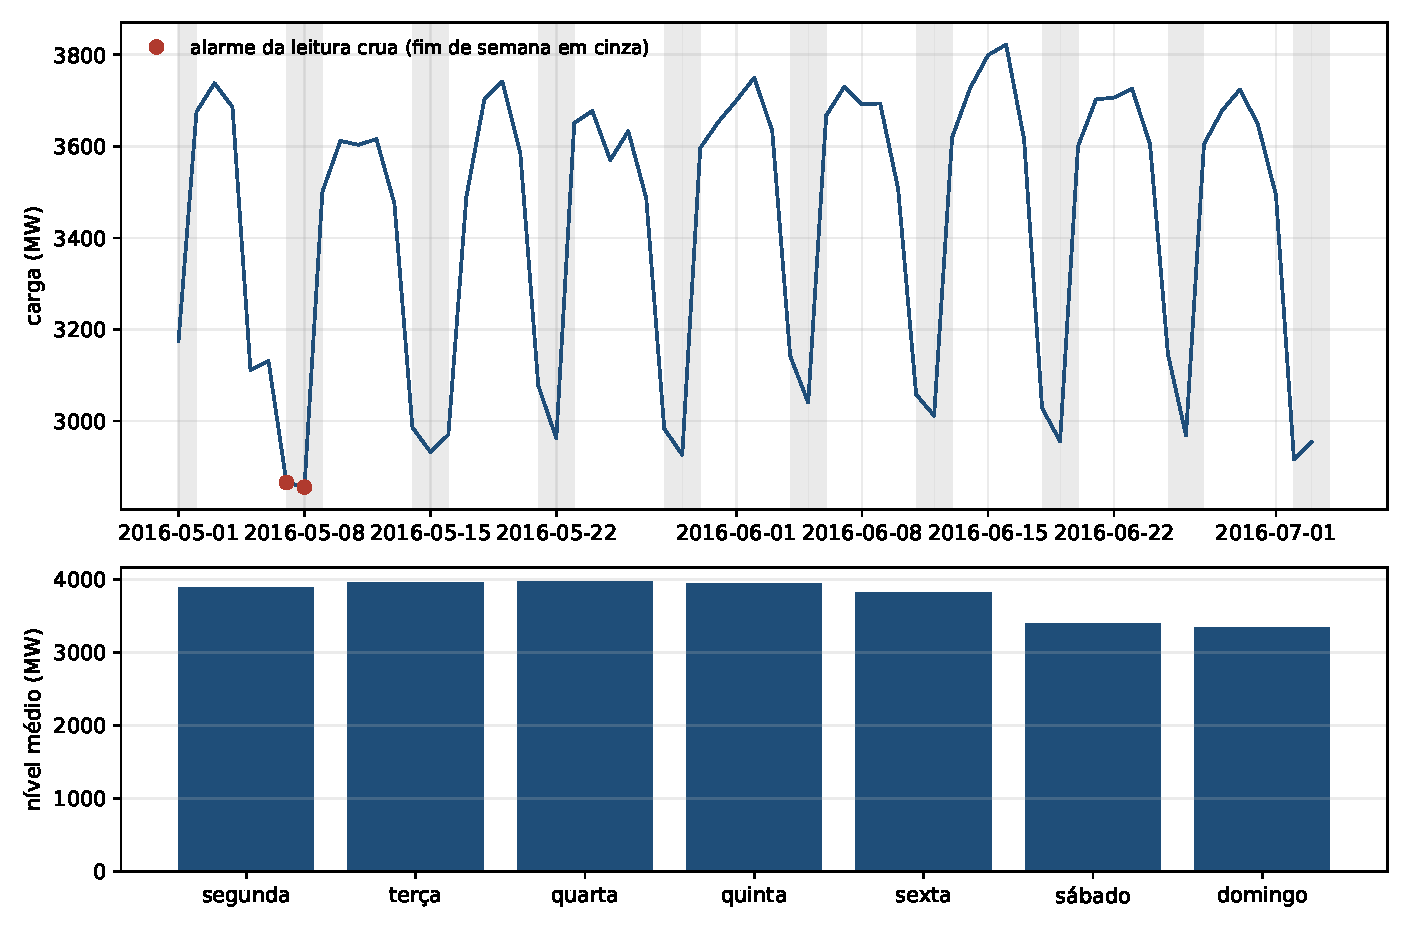
\includegraphics[width=\linewidth]{figuras/E04_calendario_1.pdf}
  \caption{Nove semanas de carga dinamarquesa. Os fins de semana estão em cinza, e os dois
    pontos são os alarmes da leitura crua: os dois caem no cinza. Embaixo, o perfil semanal
    médio dos cinco anos --- o desenho que a leitura crua estava medindo sem saber.}
  \label{fig:domingo}
\end{figure}

\begin{figure}[htbp]
  \centering
  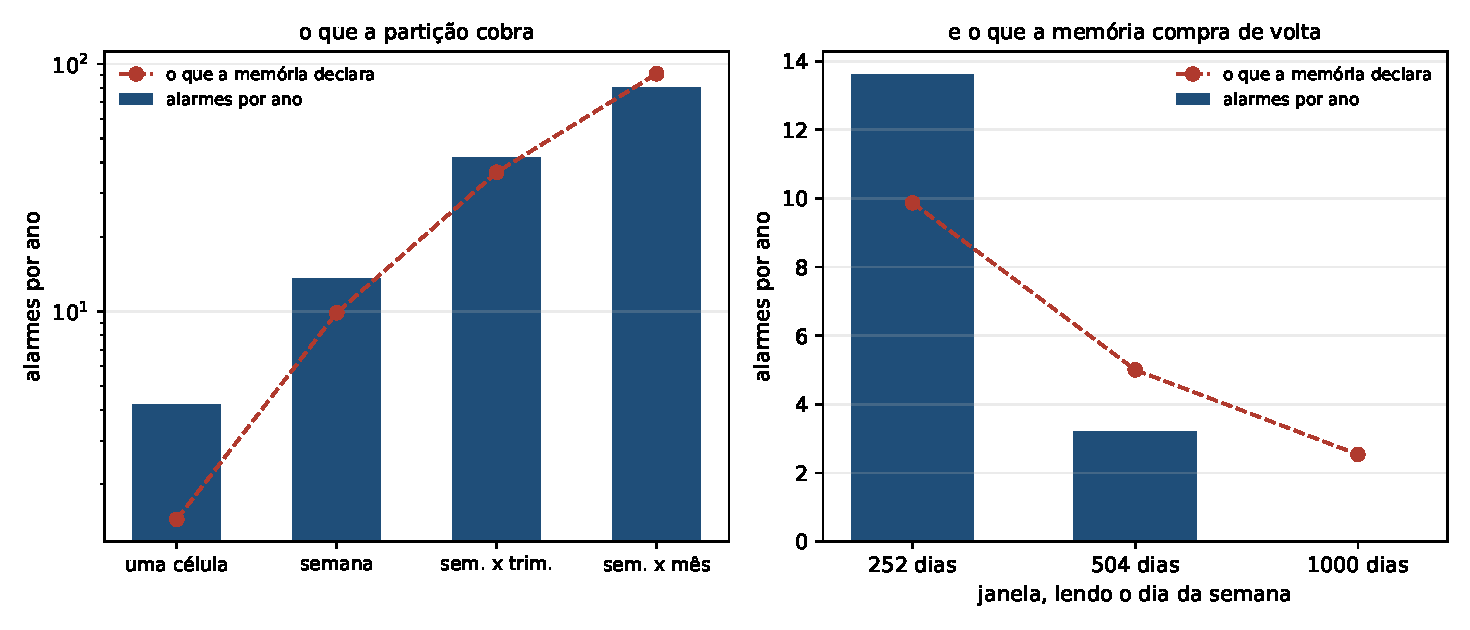
\includegraphics[width=\linewidth]{figuras/E04_calendario_2.pdf}
  \caption{À esquerda, o que a partição cobra: alarmes por ano contra o que a memória declara,
    para as quatro leituras da \cref{tab:celulas}. À direita, o que a memória compra de volta,
    com a janela crescendo e a partição semanal fixa.}
  \label{fig:particao}
\end{figure}

\section{Onde não há calendário, a partição só custa}

Falta o controle, porque a partição é uma decisão e não uma melhoria. O mesmo procedimento
aplicado ao índice acionário americano, que não tem semana, diz o que ela custa quando não há
o que ler.

Nas \numSerieDias{} observações do índice, a leitura crua dá \numCalendarioIndiceCruAlarmesAno{}
alarmes por ano contra os \numCalendarioCruPisoAno{} que a memória declara --- uma diferença de
pouco, e da mesma natureza da que o capítulo anterior discutiu. A leitura por dia da semana,
com a mesma janela, sobe para \numCalendarioIndiceSemanaAlarmesAno{} alarmes por ano, contra os
\numCalendarioIndiceSemanaPisoAno{} que a memoria declara. Nada foi
encontrado em troca: gastou-se um fator de quatro em falso alarme para descobrir que segunda
não é domingo no mercado.

A decisão fica então com a \cref{tab:perfil}. Onde a semana desenha mais de um desvio-padrão,
ler o calendário é obrigatório --- a alternativa é um vigia que relata o relógio. Onde desenha \numCalendarioAmplitudeIndice, a partição é só despesa. E o número que decide é a amplitude do perfil da série, medida.

\section{O que fica}

Fica a \textbf{célula}: o calendário é uma partição declarada dos dias, e a regra do capítulo
anterior vale dentro de cada parte, com a memória que sobra para ela. Fica também o preço, que é aritmético: $C$ células dividem a memória por $C$ e multiplicam o orçamento por $C$, e nenhuma calibração muda essa conta.

E fica o fracasso seguinte, que este capítulo tornou visível sem resolver. A partição em
células supõe que se saiba, de antemão, por onde partir os dias --- e o calendário é o caso
fácil, porque a célula está escrita no relógio. Existe uma partição que ninguém escreveu no relógio: duas séries que mudam de dependência entre si, sem que nenhuma das duas mude de
tamanho. Cada uma continua com exatamente os mesmos números, no mesmo dia da semana, e o
par delas muda tudo o que se pode perder junto. Nenhuma célula deste capítulo vê isso, e
nenhum vigia de margem também.
